\documentclass{article}

% Language setting
% Replace `english' with e.g. `spanish' to change the document language
\usepackage[english]{babel}

% Set page size and margins
% Replace `letterpaper' with `a4paper' for UK/EU standard size
\usepackage[letterpaper,top=2cm,bottom=2cm,left=3cm,right=3cm,marginparwidth=1.75cm]{geometry}

% Useful packages
\usepackage{amsmath}
\usepackage{graphicx}
\usepackage[colorlinks=true, allcolors=blue]{hyperref}


\usepackage{listings}
\usepackage{color}

\definecolor{dkgreen}{rgb}{0,0.6,0}
\definecolor{gray}{rgb}{0.5,0.5,0.5}
\definecolor{mauve}{rgb}{0.58,0,0.82}

\lstset{frame=tb,
  language=bash,
  aboveskip=3mm,
  belowskip=3mm,
  showstringspaces=false,
  columns=flexible,
  basicstyle={\small\ttfamily},
  numbers=none,
  numberstyle=\tiny\color{gray},
  keywordstyle=\color{blue},
  commentstyle=\color{dkgreen},
  stringstyle=\color{mauve},
  breaklines=true,
  breakatwhitespace=true,
  tabsize=3
}


\title{Stock Tracking Application}
\author{LT1 - Jabagat, Jasmin, Roxas, Uy}

\begin{document}
\maketitle

\begin{abstract}
The Stock Tracking Application is a terminal-based application written in Python. It mainly uses the YFinance library for the backend and the Textual library for the terminal-based GUI. Users can look up stock information, create portfolios, and manage them. 
\end{abstract}

\section{Overview}

This documentation covers the installation, usage, and functionality of the application. 

\subsection{Features}

\begin{itemize}
    \item \textbf{Real-Time Stock Lookup} - The application can fetch the latest stock data using the \textbf{yfinance} python library. 
    \item \textbf{Terminal-Based GUI} - The application presents an interactive user interface that is built using the textual Python library. 
    \item \textbf{Track multiple stocks} - The application is able to track and save multiple stocks within a portfolio. 
    \item \textbf{Simulate a trading portfolio } - The application can track and simulate a trading portfolio by tracking its market value, simulate adding and selling positions, as well as calculating gains and losses based on based on the cost average of each stock in the portfolio.
    \item \textbf{Search of Tickers - }The application has a search function that facilitates the Buy Stock function.
\end{itemize}


\section{Installation}

\subsection{Prerequisites}

Before installing the application, ensure you have installed Python 3.8 or later on your system. You will also need the following Python libraries:
\begin{itemize}
    \item \textbf{yfinance}: For fetching stock market data.
    \item \textbf{textual} - For creating the Terminal-Based GUI.
    \item \textbf{pandas}  - For operations in the application that require dataframes.
    \item \textbf{numpy} - For the required numerical computations on n dimensional arrays.
\end{itemize}


\subsection{Step-by-Step Installation}

\begin{enumerate}
    \item Clone the repository:
    \begin{lstlisting}
        git clone https://github.com/lsroxas/pds-lt1-stock-tracker
    \end{lstlisting}
    \item Create a Virtual Environment (Optional but Recommended)
    \begin{lstlisting}
        python3 -m venv venv
        source venv/bin/activate # On Windows use `venv\Scripts\activate`
    \end{lstlisting}
    \item Install Dependencies. Navigate to the application folder under the App folder:
    \begin{lstlisting}
        pip install -r requirements.txt
    \end{lstlisting}
    Alternatively, you can install the libraries individually:
    \begin{lstlisting}
        pip install yfinance textual pandas numpy
    \end{lstlisting}
    \item Run the Application
    \begin{lstlisting}
        python StockTrackerApp.py
    \end{lstlisting}
\end{enumerate}

\subsection{Navigating the Interface}


\begin{figure}
    \centering
    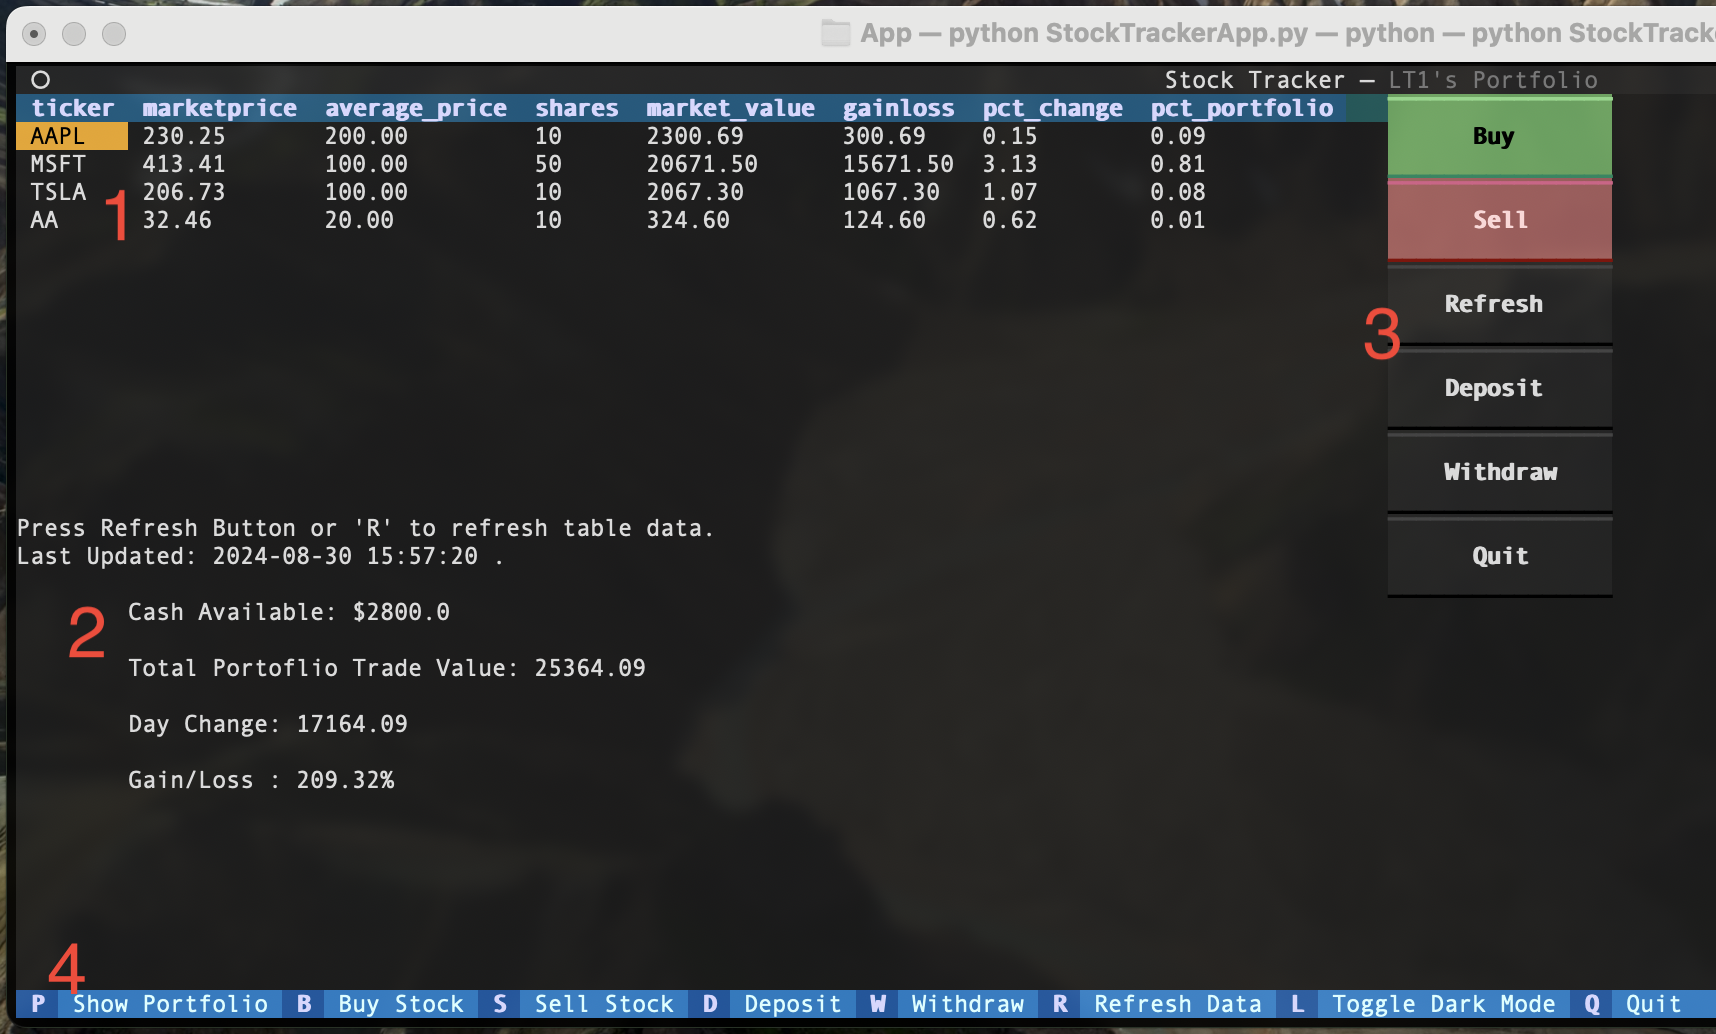
\includegraphics[width=1\linewidth]{MainWindow.png}
    \caption{Main Interface of the application}
    \label{fig:1}
\end{figure}

\begin{enumerate}
    \item \textbf{Portfolio Table}. This table contains the stocks already in your portfolio. It includes the latest market price, the average price at which all the same stocks were bought, and the gains/losses measures.
    \item \textbf{Portfolio Summary}. This contains data on when the portfolio's data was last refreshed and a summary of its value.
    \item \textbf{Main Action Buttons}. This  contains buttons that simulate actions relating to stock trading for the portfolio. 
    \item \textbf{Application Footer}. This contains keyboard shortcuts for options available within the app. 
\end{enumerate}

\subsection{Step-by-Step Installation}

Use the table and tabular environments for basic tables --- see Table~\ref{tab:widgets}, for example. For more information, please see this help article on \href{https://www.overleaf.com/learn/latex/tables}{tables}. 

\begin{table}
\centering
\begin{tabular}{l|r}
Item & Quantity \\\hline
Widgets & 42 \\
Gadgets & 13
\end{tabular}
\caption{\label{tab:widgets}An example table.}
\end{table}

\subsection{Usage}

\subsubsection{Running the Application}

\begin{enumerate}
    \item Comments can be added to your project by highlighting some text and clicking ``Add comment'' in the top right of the editor pane. To view existing comments, click on the Review menu in the toolbar above. To reply to a comment, click on the Reply button in the lower right corner of the comment. You can close the Review pane by clicking its name on the toolbar when you're done reviewing for the time being.
\end{enumerate}

Track changes are available on all our \href{https://www.overleaf.com/user/subscription/plans}{premium plans}, and can be toggled on or off using the option at the top of the Review pane. Track changes allow you to keep track of every change made to the document, along with the person making the change. 

\subsubsection{Navigating the Interface}


\subsection{How to add Lists}

You can make lists with automatic numbering \dots

\begin{enumerate}
\item Like this,
\item and like this.
\end{enumerate}
\dots or bullet points \dots
\begin{itemize}
\item Like this,
\item and like this.
\end{itemize}

\subsection{How to write Mathematics}

\LaTeX{} is great at typesetting mathematics. Let $X_1, X_2, \ldots, X_n$ be a sequence of independent and identically distributed random variables with $\text{E}[X_i] = \mu$ and $\text{Var}[X_i] = \sigma^2 < \infty$, and let
\[S_n = \frac{X_1 + X_2 + \cdots + X_n}{n}
      = \frac{1}{n}\sum_{i}^{n} X_i\]
denote their mean. Then as $n$ approaches infinity, the random variables $\sqrt{n}(S_n - \mu)$ converge in distribution to a normal $\mathcal{N}(0, \sigma^2)$.


\subsection{How to change the margins and paper size}

Usually the template you're using will have the page margins and paper size set correctly for that use-case. For example, if you're using a journal article template provided by the journal publisher, that template will be formatted according to their requirements. In these cases, it's best not to alter the margins directly.

If however you're using a more general template, such as this one, and would like to alter the margins, a common way to do so is via the geometry package. You can find the geometry package loaded in the preamble at the top of this example file, and if you'd like to learn more about how to adjust the settings, please visit this help article on \href{https://www.overleaf.com/learn/latex/page_size_and_margins}{page size and margins}.

\subsection{How to change the document language and spell check settings}

Overleaf supports many different languages, including multiple different languages within one document. 

To configure the document language, simply edit the option provided to the babel package in the preamble at the top of this example project. To learn more about the different options, please visit this help article on \href{https://www.overleaf.com/learn/latex/International_language_support}{international language support}.

To change the spell check language, simply open the Overleaf menu at the top left of the editor window, scroll down to the spell check setting, and adjust accordingly.

\subsection{How to add Citations and a References List}

You can simply upload a \verb|.bib| file containing your BibTeX entries, created with a tool such as JabRef. You can then cite entries from it, like this: \cite{greenwade93}. Just remember to specify a bibliography style, as well as the filename of the \verb|.bib|. You can find a \href{https://www.overleaf.com/help/97-how-to-include-a-bibliography-using-bibtex}{video tutorial here} to learn more about BibTeX.

If you have an \href{https://www.overleaf.com/user/subscription/plans}{upgraded account}, you can also import your Mendeley or Zotero library directly as a \verb|.bib| file, via the upload menu in the file-tree.

\subsection{Good luck!}

We hope you find Overleaf useful, and do take a look at our \href{https://www.overleaf.com/learn}{help library} for more tutorials and user guides! Please also let us know if you have any feedback using the Contact Us link at the bottom of the Overleaf menu --- or use the contact form at \url{https://www.overleaf.com/contact}.

\bibliographystyle{alpha}
\bibliography{sample}

\end{document}

